
% Preamble
\documentclass[11pt]{article}

% Packages
\usepackage{amsmath}
\usepackage{mathtools}
\usepackage{ragged2e}
\usepackage [utf8]{inputenc}
\usepackage{blindtext}
\usepackage{wrapfig}
\usepackage{xcolor}
\usepackage {polski}
\usepackage{multicol}
\usepackage[a4paper, total={5.7in, 8in}]{geometry}
\usepackage{graphicx}
\usepackage{amstex}
\usepackage{csvsimple}
\usepackage{changepage}
\usepackage{enumitem}
\usepackage[english]{babel}
\usepackage{biblatex}
\usepackage{caption}
\usepackage{indentfirst}

% Document
\begin{document}
%    Nagłówek
    \begin{flushleft}
        Filip Krauz-Damski 267 681 \hfill Data wykonania ćwiczenia:\\
        Filip Kubecki 272 655 \hfill 18 marca 2024r\\
        \hfill Data sporządzenia sprawozdania:\\
        Grupa: Pon 13:15 \hfill 24 marca 2024r\\
    \end{flushleft}
    \begin{center}
        \Large\textbf{Ćwiczenie 2.}\\
        \textbf{Oddziaływanie przyrządów na badany obiekt}
    \end{center}
    \vspace{1cm}

%    Treść
    \section{Spis przyrządów}
    \par{
        Do wykonania ćwiczenia wykorzystano:
        \begin{itemize}
            \setlength\itemsep{0em}
            \item[-] Przenośny multimetr analogowy AX-7003
            \item[-] Przenośny multimetr cyfrowy AX-588B
            \item[-] Multimetr cyfrowy Agilent 34401A
            \item[-] Zasilacz laboratoryjny symetryczny NDN DF1730SL20A
            \item[-] Rezystor dekadowy
        \end{itemize}
    }
    \section{Przebieg i cele doświadczeń}
    \noindent Doświadczenie polegało kolejno na:
    \begin{itemize}
        \setlength\itemsep{0em}
        \item Pomiarze spadków napięć wszystkimi woltomierzami na dzielniku napięcia i wyjaśnieniu różnicy wyników między przyrządami,
        \item Wyznaczeniu spadku napięcia na dzielniku w przypadku podłączenia dwóch woltomierzy równolegle oraz porównanie tej wartości z rzeczywistym pomiarem tego spadku napięcia
        \item Zmierzeniu spadków napięć na dzielniku napięcia składającego się z 4 różnych rezystorów i wytłumaczeniu czemu suma spadków tych napięć nie równa się napięciowi zasilania,
        \item Wyznaczeniu rezystancji wewnetrznej woltomierzy przy pomocy dekady rezystancyjnej,
        \item Pomiarze rezystancji wewnętrznej amperomierzy przy pomocy omomierza stosując metodę $\Omega$-2W,
    \end{itemize}
    Celem doświadczeń była obserwacja wpływu rezystancji mierników na układ pomiarowy.

    \section{Wyniki pomiarów}
    \par{
        Poniżej zostały zaprezentowane wyniki wykonanego ćwiczenia.
    }
    \subsection{Część 1 - dzielnik napięcia o wartościach 100/470[k$\Omega$]}
    \begin{center}
        \small{\textbf{Tabela 1 - spadki napięć na wszystkich miernikach}}
    \end{center}
    \begin{center}
        \csvreader[tabular = |c|c|c|c|c|,
            table head = \hline  \textbf{Miernik} & \textbf{Zakres[V]} & \textbf{Spadek napięcia[V]} & \textbf{\boldmath$R_w$[k\boldmath$\Omega$]} & \textbf{\boldmath$R_z$[k\boldmath$\Omega$]} \\\hline,
%            table foot = \hline,
            late after line = \\\hline
        ]{Dane/Czesc123.csv}{}{
            \csvcoli & \csvcolii & \csvcoliii & \csvcoliv  & \csvcolv
        }
    \end{center}

    \subsection{Część 4 - dzielnik napięcia na 4 rezystorach}
    \begin{center}
        \small{\textbf{Tabela 2 - spadki napięć na kolejnych rezystorach}}
    \end{center}
    \begin{center}
        \csvreader[tabular = |c|c|c|,
            table head = \hline  \textbf{Rezystor} & \textbf{Spadek napięcia[V]} & \textbf{Zakres[V]}  \\\hline,
%            table foot = \hline,
            late after line = \\\hline
        ]{Dane/Czesc45.csv}{}{
            \csvcoli & \csvcolii & \csvcoliii
        }
    \end{center}

    \subsection{Część 6 - Pomiar rezystancji woltomierzy przy pomocy rezystora dekadowego}
    \begin{center}
        \small{\textbf{Tabela 3 - Miernik Agilent 34401A}}
    \end{center}
    \begin{center}
        \csvreader[tabular = |c|c|c|c|,
            table head = \hline  \textbf{Zakres[V]} & \textbf{Wartość[M\boldmath$\Omega]$} & \textbf{Napięcie zasilania[V]} & \textbf{Wartość katalogowa[M\boldmath$\Omega$]}  \\\hline,
%            table foot = \hline,
            late after line = \\\hline
        ]{Dane/Czesc6Agilent.csv}{}{
            \csvcoli & \csvcolii & \csvcoliii & \csvcoliv
        }
    \end{center}

    \begin{center}
        \small{\textbf{Tabela 4 - Miernik AX-588B}}
    \end{center}
    \begin{center}
        \csvreader[tabular = |c|c|c|c|,
            table head = \hline  \textbf{Zakres[V]} & \textbf{Wartość[M\boldmath$\Omega]$} & \textbf{Napięcie zasilania[V]} & \textbf{Wartość katalogowa[M\boldmath$\Omega$]}  \\\hline,
%            table foot = \hline,
            late after line = \\\hline
        ]{Dane/Czesc6AX588B.csv}{}{
            \csvcoli & \csvcolii & \csvcoliii & \csvcoliv
        }
    \end{center}

    \newpage

    \begin{center}
        \small{\textbf{Tabela 5 - Miernik AX-7003}}
    \end{center}\vspace{-1cm}
    \begin{center}
        \csvreader[tabular = |c|c|c|c|,
            table head = \hline  \textbf{Zakres[V]} & \textbf{Wartość[K\boldmath$\Omega]$} & \textbf{Napięcie zasilania[V]} & \textbf{Wartość katalogowa[K\boldmath$\Omega$]}  \\\hline,
%            table foot = \hline,
            late after line = \\\hline
        ]{Dane/Czesc6AX7003.csv}{}{
            \csvcoli & \csvcolii & \csvcoliii & \csvcoliv
        }
    \end{center}

    \subsection{Część 7 - Pomiar rezystancji amperomierzy przy pomocy omomierza}
    \begin{center}
        \small{\textbf{Tabela 6 - Miernik Agilent 34401A}}
    \end{center}
    \begin{center}
        \csvreader[tabular = |c|c|c|,
            table head = \hline  \textbf{Zakres[V]} & \textbf{Wartość[\boldmath$\Omega]$} & \textbf{Wartość katalogowa[\boldmath$\Omega$]}  \\\hline,
%            table foot = \hline,
            late after line = \\\hline
        ]{Dane/Czesc7Agilent.csv}{}{
            \csvcoli & \csvcolii & \csvcoliii
        }
    \end{center}

    \begin{center}
        \small{\textbf{Tabela 7 - Miernik AX-588B}}
    \end{center}
    \begin{center}
        \csvreader[tabular = |c|c|c|,
            table head = \hline  \textbf{Zakres[V]} & \textbf{Wartość[\boldmath$\Omega]$} & \textbf{Wartość katalogowa[\boldmath$\Omega$]}  \\\hline,%            table foot = \hline,
            late after line = \\\hline
        ]{Dane/Czesc7AX588B.csv}{}{
            \csvcoli & \csvcolii & \csvcoliii
        }
    \end{center}

    \begin{center}
        \small{\textbf{Tabela 8 - Miernik AX-7003}}
    \end{center}
    \begin{center}
        \csvreader[tabular = |c|c|c|c|,
            table head = \hline  \textbf{Zakres[V]} & \textbf{Wartość[\boldmath$\Omega]$} & \textbf{Wartość katalogowa[\boldmath$\Omega$]}  \\\hline,%            table foot = \hline,
            late after line = \\\hline
        ]{Dane/Czesc7AX7003.csv}{}{
            \csvcoli & \csvcolii & \csvcoliii
        }
    \end{center}

    \section{Analiza wyników}
    \subsection*{Część 1-3}
    W wynikach pomiarów można zaobserwować, że spadki napięć
    zmieniają się w zależności od wykorzystanego miernika.
    Korzystając ze wzoru na dzielnik napięcia jesteśmy w stanie
    oszacować prawidłowy spadek napięcia, jaki powinniśmy otrzymać na rezystorze 470 [k$\Omega$]:
    \begin{gather*}
        U_{wyj}=U_{wej}\cdot \frac{R}{R+R_1}
    \end{gather*}
    {\footnotesize
        \begin{itemize}
            \setlength\itemsep{0em}
            \item[] \boldmath$U_{wej}$ - napięcie zasilania dzielnika napięcia,
            \item[] \boldmath$U_{wyj}$ - napięcie wyjściowe mierzone względem rezystora \textbf{R},
            \item[] \boldmath$R$ - rezystor na którym chcemy otrzymać odpowiedni spadek napięcia,
            \item[] \boldmath$R_1$ - pozostała rezystancja w obwodzie/drugi rezystor,
        \end{itemize}}

    \noindent Podstawiając dane do wzoru:
    \begin{gather*}
        U_{wyj}=U_{wej}\cdot \frac{R}{R+R_1}=10.123[V]\cdot\frac{470[k\Omega]}{470[k\Omega]+100[k\Omega]}=8.3470350877193[V]\approx 8.3470[V]
    \end{gather*}
    {\tiny\textbf{Wynik został zaokrąglony do tej samej dokładności co najdokladniejszy z wyników pomiarów w celu łatwiejszego porównania.}}\\
    \indent Można zauważyć więc że wszystkie otrzymane wyniki zostały zaniżone
    względem przewidywanej wartości. Powodem tego jest sama metoda pomiarowa.
    Wstawiając do układu woltomierz tak jak na schemacie niżej (woltomierz symbolizuje
    rezystancja 10 [M$\Omega$] – rezystancja wewnętrzna miernika Agilent 34401A),
    zmieniamy rezystancje całego układu.
    \begin{center}
        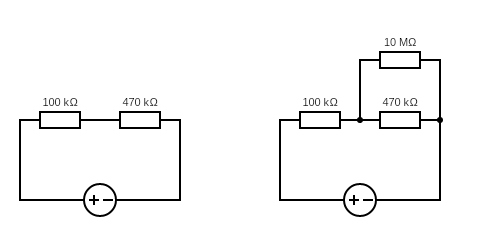
\includegraphics[scale = 0.5]{F:/Projekty Intellij/Text/Metrologia/Ćwiczenie2/Img/Circ1.png}
    \end{center}
    Największą różnicę otrzymaliśmy na mierniku analogowym AX-7003 ponieważ posiada on
    najmniejszą rezystancję wewnętrzną co znacząco zaniża mierzony spadek napięcia.\\
    Dzięki znajomości rezystancji wewnętrznej mierników jesteśmy w stanie wyliczyć
    rezystancję zastępczą na której wykonujemy pomiar spadku napięcia przy dołożeniu woltomierza do układu.
    Wynika ona bowiem z rezystancji zastępczej dwóch rezystorów połączonych równolegle:
    \begin{gather*}
        R_z=\frac{R_1\cdot R_2}{R_1+R_2}
    \end{gather*}
    Na przykładzie miernika Agilent 34401A włączonego równolegle do rezystora 470[k$\Omega$]:
    \begin{gather*}
        R_z=\frac{R_1\cdot R_2}{R_1+R_2}=\frac{470[k\Omega] \cdot 10[M\Omega]}{470[k\Omega]+10[M\Omega]}=448901.623\dots [\Omega]
    \end{gather*}
    \indent Idąc dalej jesteśmy w stanie obliczyć przewidywaną wartość naszych pomiarów podstawiając
    tą rezystancję do wzoru na spadek napięcia w dzielniku napięcia. Poniżej zostały przedstawione
    wynik tych obliczeń na przykładzie dwóch mierników Agilent 34401A włączonych równolegle do rezystora 470[k$\Omega$]:
    \begin{gather*}
        U_{wyj}=U_{wej}\cdot \frac{R}{R+R_1}=10.123[V]\cdot \frac{429616\dots[\Omega]}{429616\dots[\Omega]+100[k\Omega]}=8.21162\dots[V]
    \end{gather*}
    \newpage
    Poniżej przedstawiono tabelę z wszystkimi otrzymanymi wynikami.
    \begin{center}
        \csvreader[tabular = |c|c|c|c|c|,
            table head = \hline  \textbf{Wartość zmierzona[V]} & \textbf{Wartość obliczona[V]} & \textbf{$R_z$[$\Omega$]} & \textbf{$\Delta_V$[V]} & \textbf{$\delta_V$[\%]} \\\hline,
%            table foot = \hline,
            late after line = \\\hline
        ]{Dane/Wyniki1.csv}{}{
            \csvcoli & \csvcolii & \csvcoliii & \csvcoliv  & \csvcolv
        }
    \end{center}
    {\footnotesize
        \begin{itemize}
            \setlength\itemsep{0em}
            \item[] \boldmath$R_z$ - rezystancja zastępacz układu woltomierz rezystor 470[k$\Omega$],
            \item[] \boldmath$\Delta_V$ - błąd bezwzględny wartości zmierzonej dla kolejnych mierników,
            \item[] \boldmath$\delta_V$ - błąd względny wartości zmierzonej dla kolejnych mierników,
        \end{itemize}}
    Jak widzimy w tabeli powyżej wszystkie wartości zmierzone albo zawierają
    się w wartości obliczonej w granicy błędu pomiarowego miernika albo różnica
    między wartościami jest na tyle niewielka że może wynikać z dodatkowej
    oporności przewodów pomiarowych czy niedokładności rezystancji samych rezystorów.

    \subsection*{Część 4-5}
    Doświadczenie zostało błędnie przeprowadzone gdyż napięcie zasilania zostało zmierzone raz na
    początku ustawiania układu a nie mierzone ciągle tak jak zostało zapisane w poleceniu.
    Mimo wszystko jesteśmy w stanie wyciągnąć częściowe wnioski wynikające z ćwiczenia.\\
    \indent Po zsumowaniu spadków napięć na wszystkich rezystorach otrzymano wartość 10.002847[V].
    Napięcie zasilania wynosiło 10.12[V] więc różnica tych dwóch wyników wyniosła 0.117153[V].
    Jest to wynik którego można było się spodziewać gdyż zachodzi tutaj zjawisko przedstawione w poprzedniej części ćwiczenia.
    Gdy podłączamy woltomierz na zaciski rezystora zmieniamy rezystancję elementu na którym mierzymy spadek napięcia jak i rezystancję całego układu.
    Skutkiem tego jest zaniżenie wartości mierzonych przez rezystancję wewnętrzną woltomierza.\\
    \indent Jesteśmy w stanie wy syntetyzować idealny wynik przeprowadzonego doświadczenia korzystając
    ze wzoru na rezystancje zastępczą układu równoległego rezystorów oraz z wzoru na dzielnik napięcia.
    Zakładając idealne zasilanie 10[V], rezystory o idealnych wartościach 1k[$\Omega$], 10k[$\Omega$],
    100k[$\Omega$], 1M[$\Omega$] oraz idealnej wartości rezystancji wewnętrznej woltomierza równej 10M[$\Omega$] możemy wyliczyć poniższe wartości:
    \begin{center}
        \csvreader[tabular = |c|c|c|c|,
            table head = \hline  \textbf{$R$[$\Omega$]} & \textbf{$U_R$[V]} & \textbf{$R_z$[$\Omega$]} & \textbf{$U_{R_z}$[V]} \\\hline,
%            table foot = \hline,
            late after line = \\\hline
        ]{Dane/Wyniki4.csv}{}{
            \csvcoli & \csvcolii & \csvcoliii & \csvcoliv
        }
    \end{center}
    {\footnotesize
        \begin{itemize}
            \setlength\itemsep{0em}
            \item[] \boldmath$R$ - rezystancja rezystora,
            \item[] \boldmath$R_z$ - rezystancja zastępcza układu rezystor/woltomierz,
            \item[] \boldmath$U_R$ - spadek napięcia na rezystorze,
            \item[] \boldmath$U_{R_z}$ - spadek napięcia na układzie rezystor/woltomierz,
        \end{itemize}}
    \indent Po zsumowaniu spadków napięć $U_{R_z}$ otrzymujemy
    wartość 9.902754713[V]. Po odjęciu od napięcia zasilania
    otrzymujemy wartość 0.097245287[V].
    Wartość ta jest zbliżona do wartości zmierzonej jednak różnica ta
    nie mieści się w granicy błędu pomiarowego z powodów wymienionych na początku tej sekcji.

    \subsection*{Część 6}
    Dla miernika Agilent 34401A wyniki (Tabela 3) są zbliżone
    do wartości katalogowych a różnica między wartościami mieści się w granicy około 1\%.\\
    \indent Taka sama sytuacja występuje w przypadku miernika AX-588B gdzie
    różnica między notą katalogową a wartością wyznaczoną przy użyciu dekady rezystancyjnej mieści się w granicach błędu.
    Nie udało się jednak zmierzyć rezystancji zakresu 1000[V] na
    tym mierniku gdyż zakres ten pozwala na odczyt z dokładnością do jedności
    a poprawne wyznaczenie rezystancji wymagało możliwości odczytu wartości napięcia z dokładnością do jednej dziesiątej.
    Wartość ta została więc pominięta w tabeli z wynikami (Tabela 4).\\
    \indent Inaczej mają się wyniki miernika analogowego AX-7003. W jego przypadku
    im wyższy zakres mierzono tym większa różnica wyniku od wartości katalogowej.
    Jest to bezpośredne następstwo charakterystyki niepewności mierników analogowych
    które najdokładniej mierzą wartości bliskie końca zakresu.
    W tej sytuacji wartości znajdowały się poniżej $\frac{1}{4}$ skali co wpłynęło znacząco na pomiary.
    Tak samo jak w przypadku miernika AX-588B nie udało się dokonać
    pomiaru na najwyższym zakresie gdyż dokładność skali miernika nie pozwalała na odczyt wartości 2.5[V] na zakresie 500[V].
    Wartość ta nie została więc uwzględniona w tabeli z wynikami (Tabela 5).\\
    \indent Poniżej zostały umieszczone wartości niepewności bezwzględnej($\Delta$) i względnej($\delta$) miernika AX-7003 dla danego doświadczenia:
    \begin{center}
        \csvreader[tabular = |c|c|c|c|c|,
            table head = \hline  \textbf{Zakres[V]} & \textbf{Spadek napięcia na mierniku[V]} & \textbf{$\Delta$[V]} & \textbf{\boldmath$\delta$[\%]} \\\hline,
%            table foot = \hline,
            late after line = \\\hline
        ]{Dane/Wyniki2.csv}{}{
            \csvcoli & \csvcolii & \csvcoliii & \csvcoliv
        }
    \end{center}
    Tak jak widać różnice w wartościach wynikają z niepewności pomiarowej miernika analogowego.

    \newpage

    \subsection*{Część 7}
    Przy pomocy miernika Agilent 34401A stosując metodę $\Omega-2W$(Two wire)
    wykonano pomiary rezystancji wszystkich amperomierzy na wszystkich zakresach stałoprądowych.
    W celu poprawnej analizy wyników na początku wyliczono niepewności pomiaru rezystancji przy pomocy miernika Agilent 34401A.
    Niepewność ta dana jest wzorem:
    \begin{gather*}
        \Delta=\pm(a\%\cdot X+c\%\cdot X_{max})
    \end{gather*}
    {\footnotesize
        \begin{itemize}
            \setlength\itemsep{0em}
            \item[] \boldmath$a$ - składowa niepewności wynikająca tolerancji wartości elementów, nieliniowości, wzmocnienia i niepewności wzorca napięcia,
            \item[] \boldmath$c$ - składowa niepewności wynikająca z rozdzielczości przetwarzania sygnału analogowego na cyfrowy - błąd kwantowania i zliczania,
            \item[] \boldmath$X$ - wartość odczytana,
            \item[] \boldmath$X_{max}$ - zakres pomiarowy (największa możliwa do zmierzenia wartość),
        \end{itemize}}
    Dodatkowo producent podaje że dla metody $\Omega-2W$ należy dodać wartosć 0.2[$\Omega$] w
    przypadku gdy nie została użyta funkcja \textbf\textit{NULL}. Jest to działanie
    które ma za zadanie usunąć rezystancję przewodów z odczytanej wartości. W przypadku
    tego pomiaru nie została użyta funkcja \textbf\textit{NULL} a przewody zastosowane w
    doświadczeniu nie były przewodami dostarczonymi przez firmę Keysight wraz z ich urządzeniem.\\
    Przykładowy pomiar niepewności rezystancji dla amperomierza Agilent 34401A(zakres badanego amperomierza Agilent 34401A 0.1[A]):
    \begin{gather*}
        \Delta=\pm(a\%\cdot X+c\%\cdot X_{max})=\pm(0.003\%\cdot 5.507[\Omega]+0.003\%\cdot 100[\Omega]+0.2[\Omega])=\pm 0.203165\dots[\Omega]
    \end{gather*}
    \noindent Poniżej zostały podane niepewności dla kolejnych mierników oraz ich zakresów:
    \begin{center}
        \csvreader[tabular = |c|c|c|c|c|,
            table head = \hline  \textbf{Miernik} & \textbf{Badany zakres[A]} & \textbf{Zakres omomierza[$\Omega$]} & \textbf{\boldmath$\Delta$[$\Omega$]} & \textbf{\boldmath$\delta$[\%]} \\\hline,
%            table foot = \hline,
            late after line = \\\hline
        ]{Dane/Wyniki3.csv}{}{
            \textbf{\csvcoli} & \csvcolii & \csvcoliii & \csvcoliv & \csvcolv
        }
    \end{center}\vspace{3mm}
    \indent Można zauważyć że dla zakresów mierzących niewielkie prądy wartości mierzone i dane w notach katalogowych
    są do siebie zbliżone (Tabela 6,7,8) co pokazują również niepewności względne. Jednak dla zakresów mierzących duże prądy wyniki rozbiegają się.
    Przyczyną takiego stanu rzeczy jest prawdopodobnie użycie przewodów o nieznajomej
    rezystancji oraz nie użycie funkcji \textbf{\textit{NULL}} na omomierzu przed przystąpieniem do pomiarów.\\
    \indent Dodatkowo zaznaczamy że producent nie podał wartości rezystancji
    wewnętrznej dla miernika AX-7003 na pomiarze prądu. Tak
    samo wartość ta nie została bezpośrednio przedstawiona w
    nocie katalogowej miernika AX-588B. Została tam jednak podana
    wartość maksymalnego spadku napięcia na wszystkich zakresach która wynosiła 0.2[V].
    Korzystając z prawa Ohma wykorzystano tą wartość do oszacowania wartości rezystancji wewnętrznej amperomierza tak jak przedstawiono poniżej:
    \begin{gather*}
        R=\frac{U}{I_{max}}
    \end{gather*}
    {\footnotesize
        \begin{itemize}
            \setlength\itemsep{0em}
            \item[] \boldmath$R$ - rezystancja wewnetrzna amperomierza na danym zakresie,
            \item[] \boldmath$U$ - maksymalny spadek napięcia na zakresie wynoszący 0.2[V].
            \item[] \boldmath$I_{max}$ - maksymalny prąd/zakres pomiarowy,
        \end{itemize}}
    \noindent Przykładowo dla zakresu 0.02[A]:
    \begin{gather*}
        R=\frac{U}{I_{max}}=\frac{0.2[V]}{0.02[A]}=10[\Omega]
    \end{gather*}

    \section{Uwagi i wnioski}
    Z całego ćwiczenia można wywnioskować że rezystancja urządzeń
    pomiarowych może mieć duży wpływ na ostateczny wynik pomiaru.
    Należy więc przed przystąpieniem do mierzenia danej wartości
    zastanowić się czy zastosowane urządzenia nie wpłyną negatywnie na wynik doświadczenia.
    W przypadku woltomierzy należy szczególnie uważać przy pomiarze
    spadków napięcia na bardzo dużych rezystancjach gdyż rezystancja zastępcza
    takich układów może znacznie się zmniejszyć co poda zaniżony wynik pomiaru.\\
    \indent Dodatkowo z ostatnich dwóch części ćwiczenia można zauważyć że dla woltomierzy wraz ze
    wzrostem ich zakresu powinna rosnąć ich rezystancja wewnętrzna a w przypadku amperomierzy przeciwnie(chyba że miernik na wszystkich zakresach posiada jednakową bardzo dużą rezystancje wewnętrzną),
    im większy zakres tym mniejsza powinna być rezystancja miernika.


\end{document}